\begin{solution}
	The answer is 26. You can find an example of 5 cuts that divide the cake into 26 pieces here: \url{https://www.desmos.com/3d/baf22a25f7}.\\[0.2cm]
	\begin{center}
	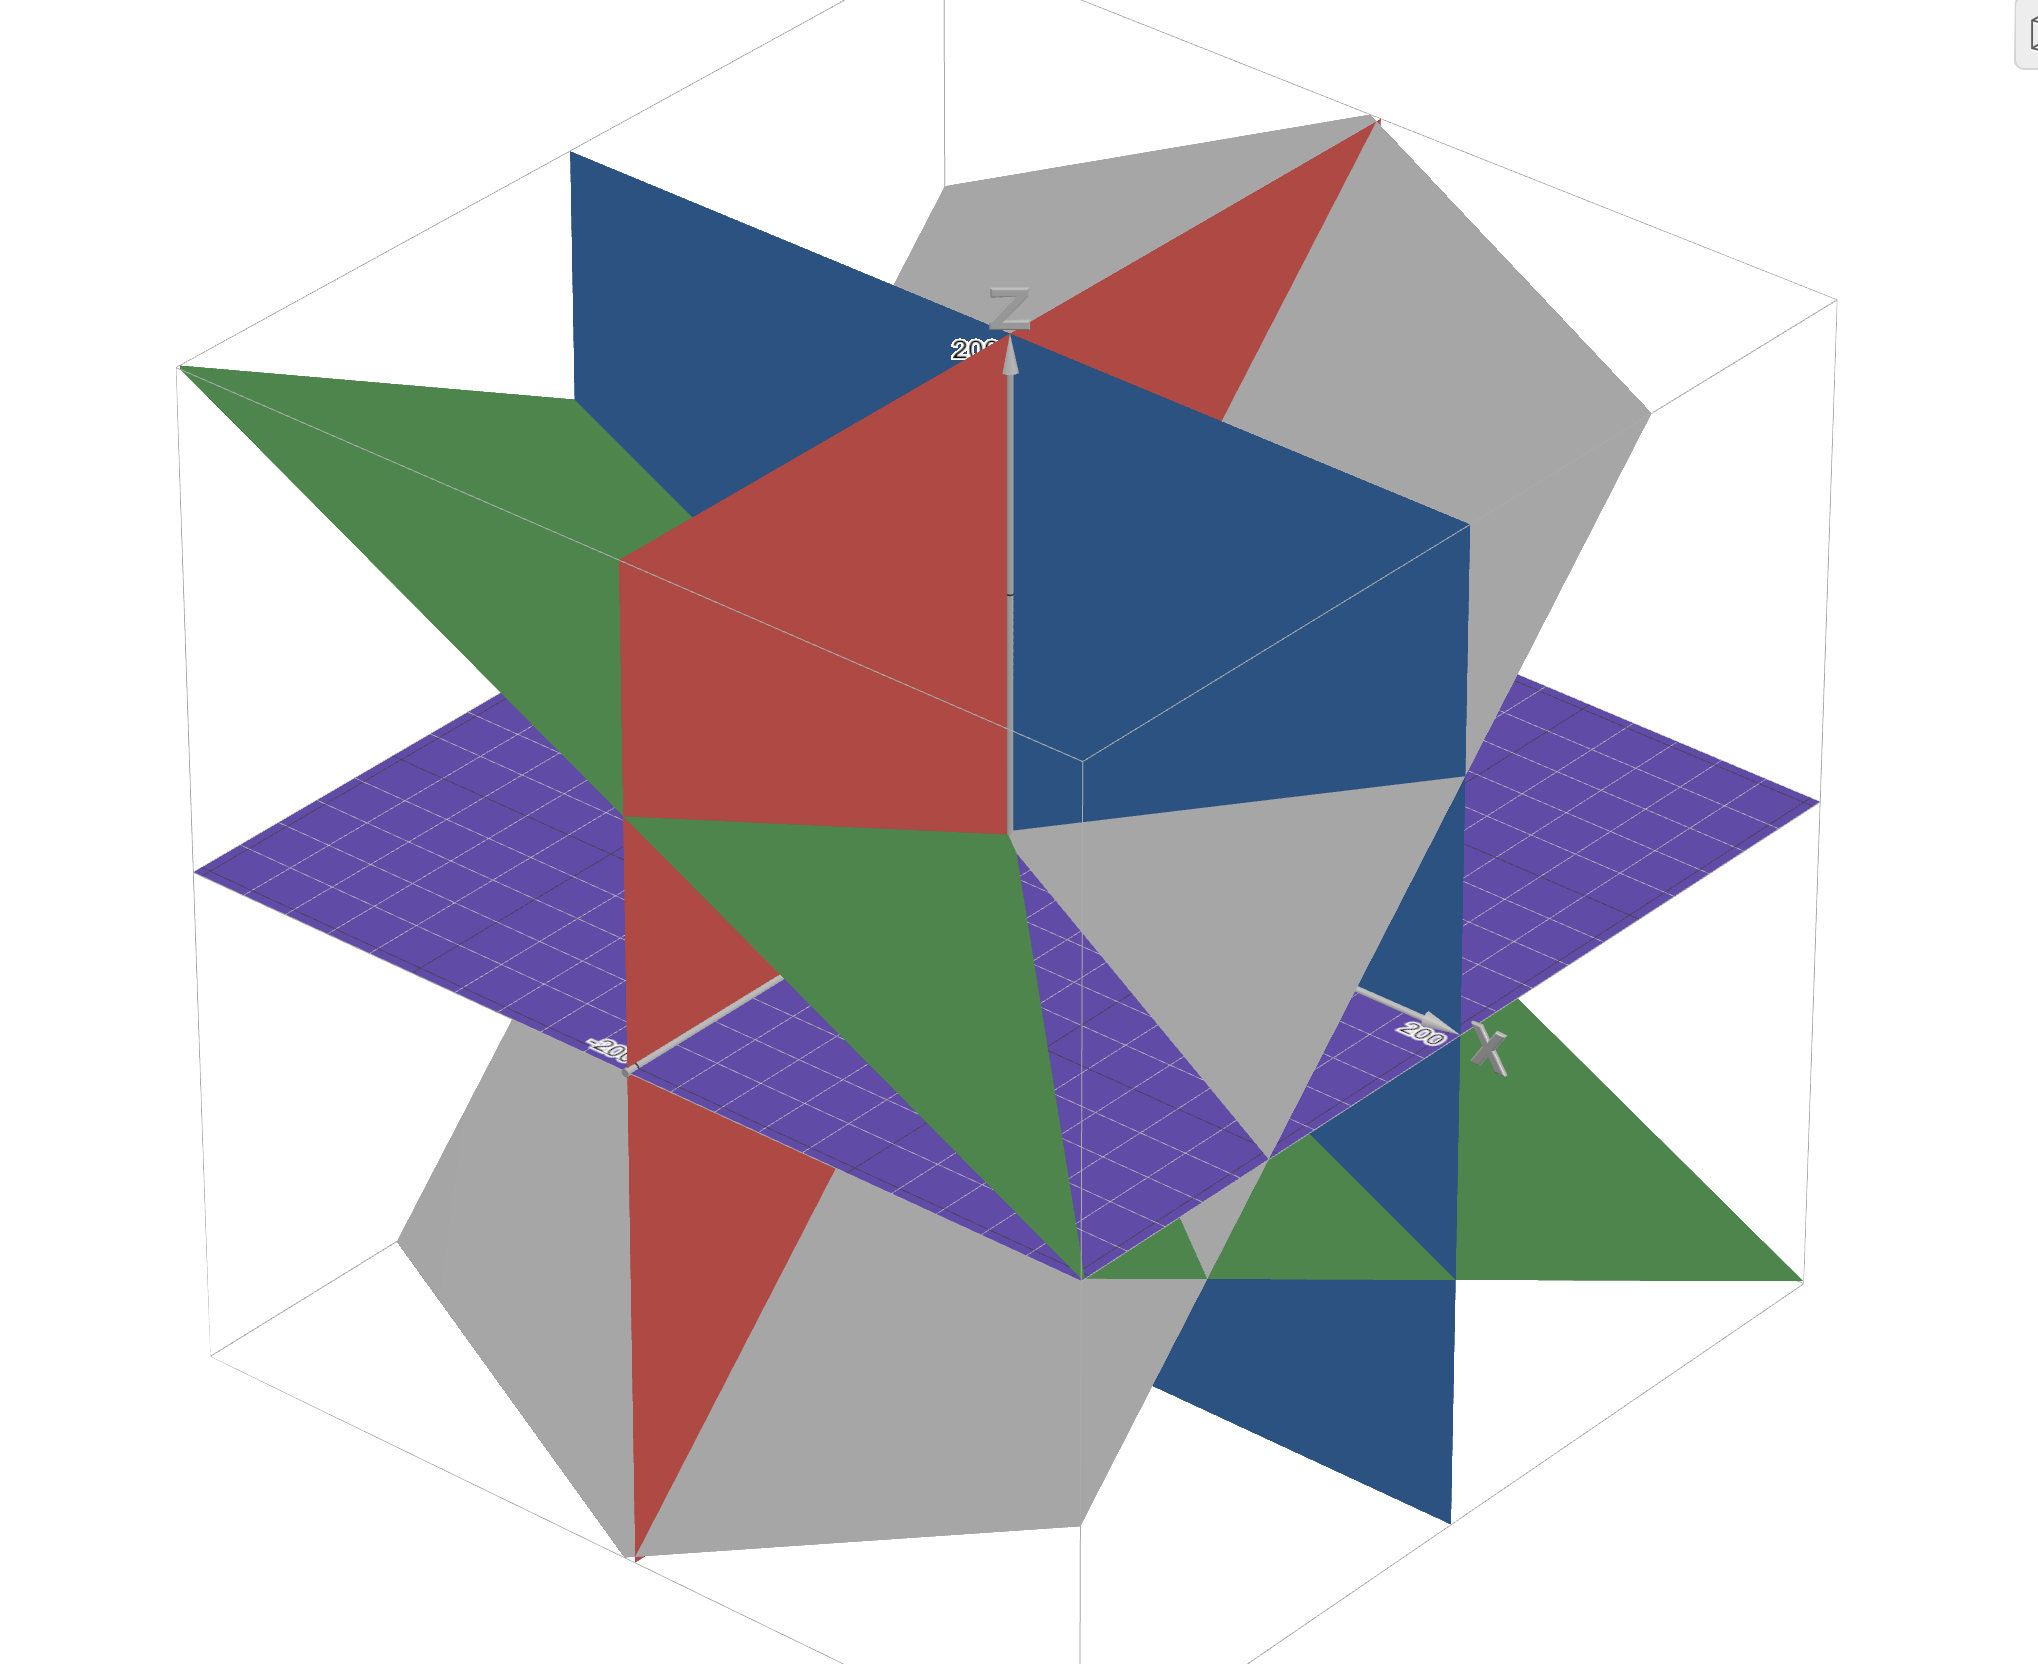
\includegraphics[width=9cm]{58/figs/58_sol.png}
	\end{center}
	Next, we will discuss why the cake cannot be cut into more than 26 pieces with 5 cuts. To do this, we first solve the 2D version of the problem. Let $L(n)$ be the maximum number of parts of a plane divided via $n$ lines. When we add the $n$'th line to the plane, it cuts the previous lines at at most $n-1$ places, so it adds at most $n$ new parts to the plane. Therefore
	\begin{itemize}
		\item $L(0)=1$
		\item $L(1)=L(0)+1=2$
		\item $L(2)=L(1)+2=4$
		\item $L(3)=L(2)+3=7$
		\item $L(4)=L(3)+4=11$
	\end{itemize}
	
	Now for the 3D version, we denote the number of the maximum parts of a cake with n cuts by $P(n)$.
	
	After the $n$'th cut, the intersection of the $n-1$ previous planes with this one forms at most $n-1$ lines. Thus the previous planes create at most $L(n-1)$ 2D parts on the new plane. Each of these 2D parts can be the cross-section of one of the 3D pieces. So the $n$th cut intersects with at most $L(n-1)$ 3D pieces of the previous cuts. Therefore $ P(n)=P(n-1)+L(n-1)$. Therefore:
	\begin{itemize}
		\item $P(0)=1$
		\item $P(1)=P(0)+L(0)=2$
		\item $P(2)=P(1)+L(1)=4$
		\item $P(3)=P(2)+L(2)=8$
		\item $P(4)=P(3)+L(3)=15$
		\item $P(5)=P(4)+L(4)=26$
	\end{itemize}
	This implies that  $P(5)=26$. Therefore, the maximum number of pieces of the cake after 5 cuts is 26.
\end{solution}
